\section{Remote Attestation}
\label{sec:remote-attestation}

Remote attestation is the process that allows a remote party to verify the
trustworthiness of a device or platform. \citetitle{rfc9334} \cite{rfc9334}
provides a standardized framework for remote attestation, which defines various
roles, protocols, and data structures involved in this process. This section
will provide an overview of the remote attestation process.

\begin{figure}[H]
  \centering
  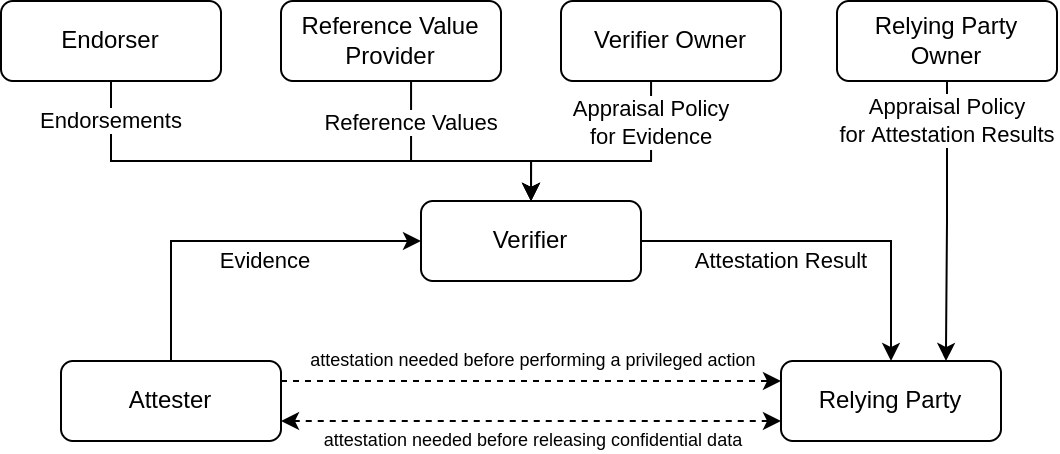
\includegraphics[width=0.8\linewidth]{resources/rats-data-flow.drawio.png}
  \caption{Remote attestation roles and data flow.}
  \label{fig:rats-data-flow}
\end{figure}


The remote attestation process begins with the relying party requesting a
verification of the attester. Subsequently, the attester generates evidence
about its trustworthiness, which is used by the verifier in combination with
endorsements from endorsers and reference values from reference value providers
by applying appraisal policies to assess the trustworthiness of the attester,
producing attestation results. The relying party then applies its own appraisal
policy to make an application-specific decision, such as performing a privileged
action or releasing confidential data to the attester. This process is
illustrated by Figure \ref{fig:rats-data-flow}.

We will assume that the verifier has already established trust and a secure
communication channel with the relying party. RATS outlines how the trust
between those two roles can be established \cite[Section~7.1]{rfc9334}

\subsection{Chain of Trust}
\label{sec:ra-chain-of-trust}

\begin{figure}[H]
  \centering
  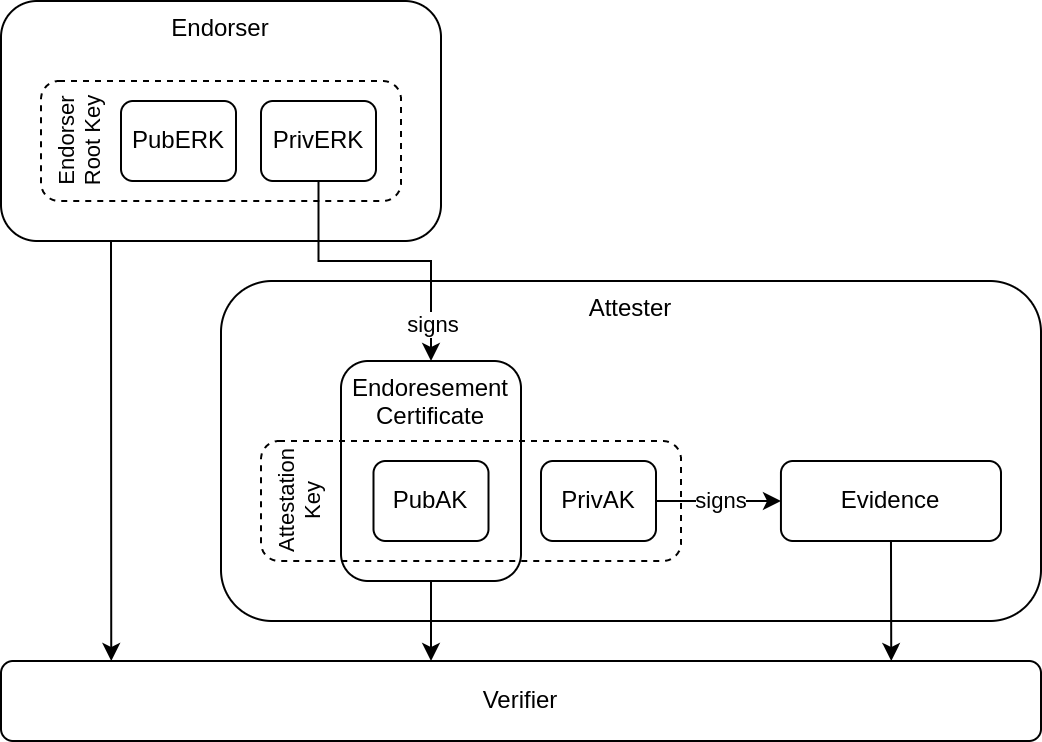
\includegraphics[width=0.7\linewidth]{resources/ra-chain-of-trust.drawio.png}
  \caption{Remote attestation chain of trust.}
  \label{fig:ra-chain-of-trust}
\end{figure}

Typically, a verifier comes to trust an attester indirectly by having an
endorser, creating a chain of trust. This chain of trust is rooted at the
endorser root key. The endorser provisions each attester with an attestation
key, which is used to sign evidence. At the very least, the private part of the
attestation key has to be stored in tamper-proof hardware, in order to prevent
unauthorized access to the key. The endorser then issues an endorsement
certificate which includes the public attestation key and signs the certificate
using its own private endorsement root key.

The endorsement certificate represents the endorsement from the endorser that
the attester can be trusted. Both the endorsement certificate and the public
part of the endorser root key have to be provided to the verifier. Before
starting its first verification, the verifier has to authenticate the
endorsement certificate by validating its signature using the public endorser
root key.

Evidence produced by the attester is signed by the attester using the
attestation key. After receiving evidence from the attester, the verifier first
verifies that the evidence was produced by the attester by validating its
signature using the public attestation key, which is included in the endorsement
certificate. Subsequently, the verifier confirms the integrity of the evidence
using the validated signature.

After validating the authenticity and integrity of the evidence, the verifier
appraises the evidence using reference values provided by the reference
provider.

\subsection{Secure Communication Channel between Attester and Relying Party}
\label{sec:ra-secure-communication-channel}

\begin{figure}[H]
  \centering
  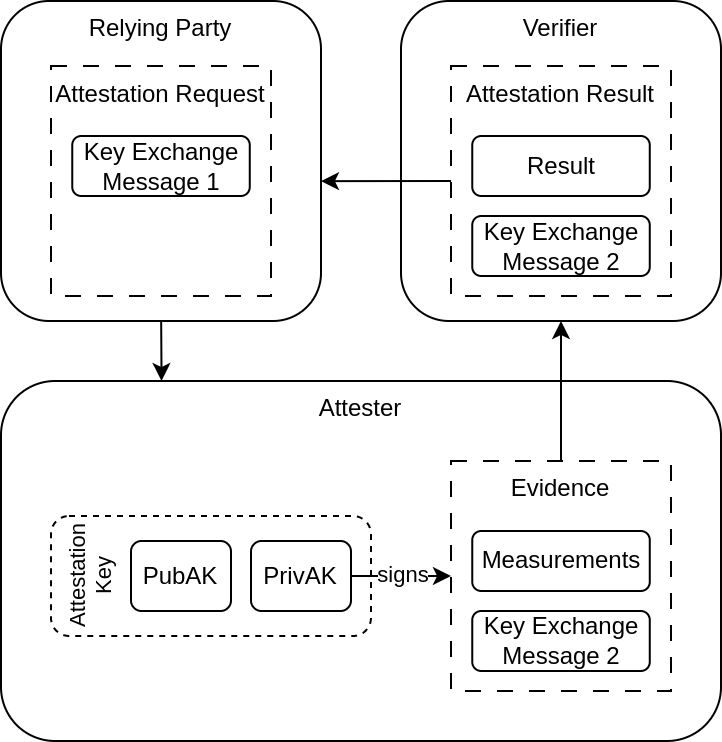
\includegraphics[width=0.5\linewidth]{resources/ra-key-exchange.drawio.png}
  \caption{Integration of the Diffie-Hellman key exchange protocol into the remote attestation process.}
  \label{fig:ra-key-exchange}
\end{figure}

The remote attestation process can also be used to establish a secure
communication channel between the attester and the relying party. This can be
achieved by integrating a key agreement protocol into the remote attestation
process. This section will outline how a secure channel can be established
between the attester and the relying party using the Diffie-Hellman key exchange
as an example (see Section \ref{sec:key-agreement}). We will assume that the
prime number $p$ and generator $g$ are already specified by the protocol or are
already agreed upon.

The relying party starts the attestation process, by requesting a verification
of the attester. In the request the relying party includes the first key
exchange message. The attester then produces evidence which includes the second
key exchange message. Because the evidence is signed by the attestation key it
is part of the chain of trust, allowing the verifier to validate the
authenticity and integrity of the key exchange message. After a successful
verification the verifier includes the key exchange message in the attestation
result. Now both the attester and the relying party have exchange their key
exchange messages, which included $pub_A$ and $pub_B$, allowing the derivation
of a shared secret key $K$ that can be used to establish a secure communication
channel between both parties.

A man-in-the-middle attack between the attester and the verifier can easily be
detected, because modification of the key exchange message would result in the
verification of the integrity of the evidence to fail.

While the previous illustration is about the integration of the establishment of
a secure communication channel into the remote attestation process, current
ongoing work by \citeauthor{fossati-tls-attestation-02}
\cite{fossati-tls-attestation-02} proposes the reverse, integration of the
remote attestation process into the already well established TLS protocol.
